\section{GTAC modelling}
In the GTAC anechoic chamber there is a 96-loudspeaker array distributed as an irregular octagon in the horizontal plane (\autoref{WFSdistribution}), $1.65 \si{m}$ above the floor, with a separation between loudspeakers of $\secondarySourceSeparation = 0.18 \si{m}$. 

\begin{figure}
	\centering
	\reflectbox{\rotatebox[origin=c]{180}{
			\includegraphics[height=0.3\textheight]{./Img/WFSarraySchemeReport.pdf}
	}}
	\caption[WFS array distribution]{Schematic of the GTAC loudspeaker array distribution}
	\label{WFSdistribution}
\end{figure}

Many variables have an impact on the acoustic field generated by the loudspeakers: frequency dependent directivity of each individual loudspeaker, non-linearities, reverberation of the chamber, diffraction, reflections on the floor (which is not recovered with absorbing material as the walls), etc. However, if we assume a simple model where the anechoic chamber is perfectly configured to emulate free-space conditions, and every loudspeaker is identical to the rest and behaves as an ideal monopole, then the similarities with the scenario presented by WFS theory become clear.

Under ideal conditions, the octagon can be interpreted as the closed curve of secondary sources $\sectionTheo$ discretized with a step of $\secondarySourceSeparation = 0.18 \si{m}$, so the aliasing frequency for a speed of sound $c = 340 \si{m/s}$ is $f_\mathit{alias} = 944.44\si{Hz}$.  As we only count with monopole sources (loudspeakers with dipole characteristics are more difficult and expensive to manufacture), we should use the Rayleigh 2.5D I integral (\autoref{RayleighI2.5}), but $\sectionTheo$ should be an infinite line and not an octagon. Of course, an infinite array is not realizable in practice, so at some point we must truncate the array anyway. On the other hand, when dealing with a bent array, the amplitude factor $g = \sqrt{\frac{d}{d + \abs{\PosTheo[primarySource][z]}}}$ that was calculated when $\sectionTheo$ was a straight line might not be the best option any more.

The actual loudspeaker feeding signals that were used, were calculated applying formulas that were provided by the professors and are particularized for the specific geometry of the GTAC array:
\begin{equation}
\begin{aligned}
g &= 
\begin{cases}
\sqrt{\frac{\distLinePoint}{\distLinePrimSource + \distLinePoint}} & \normPrimaryPropAngle \leq 90^\circ \\
0 & \normPrimaryPropAngle > 90^\circ
\end{cases}
\\
\distLinePoint &= \frac{1.44}{2} + 1.44 \cos\left( \frac{\pi}{4} \right)
\end{aligned}
\label{amplitFactorGTAC}
\end{equation}
where $\normPrimaryPropAngle$ and $\distLinePrimSource$ are represented in
\autoref{figAngleCondition}.

For simplification purposes, from now on it will be assumed that primary sources are monopoles.

\section{Introduction to simulations}
Traditionally, WFS has been used, not to cancel noise, but as a spatial audio reproduction system that competes with existing stereophonic systems as Dolby Surround. The main focus has been, then, not in replicating accurately a field, but in generating the subjective impression of natural hearing, this is, of sound heard from various directions. So, the evaluation of performance has been usually guided by the ability of subjects to localize virtual sound sources and other subjective measures.

Since human hearing has limitations, there are objective sound characteristics that it cannot perceive. We can take advantage of this, and use compression, downsampling and other techniques (common in mp3 and other compression formats) that lower the requirements of the system without worsening the subjective perception. One thing that humans cannot distinguish is constant phase shift with frequency. So, when implementing WFS, the term $\sqrt{j}$ can be omitted (as done in the real implementations in \cite{Verheijen} and \cite{Vogel}) since it would require the implementation of a FIR filter that wouldn't add anything to the experience of the audience. Depending on the requirements of the system, the frequency dependent coefficient $\sqrt{k}$ can also be omitted, with the disadvantage that it would produce coloration of the sound (\cite{Vogel}).

Without both filters, the signal of a given loudspeaker can be calculated by just applying a delay to the virtual source signal and multiplying it by a scalar.
\begin{gather}
\signal[wfs][frequency](f) = \signal[nsVirt][frequency](f) \cos\normPrimaryPropAngleSection \frac{e^{-jk\distLinePrimSource}}{\sqrt{\distLinePrimSource}} g
\\
\signal[wfs][time](t) = \signal[nsVirt][time](t) \frac{g \cos\normPrimaryPropAngleSection}{\sqrt{\distLinePrimSource}}
\ast\delta(t - \distLinePrimSource/c)
\label{wfsSignalTime}
\end{gather}
where $\signal[nsVirt][time](t) = -\signal[ns][time](t)$ is the signal transmitted by the primary source, now called virtual noise source because it is the same as the signal transmitted by the noise source multiplied by $-1$.
\begin{figure}
	\centering
	\def\svgwidth{0.4\columnwidth}
	\graphicspath{{Img/}}
	\input{Img/WFSParameters.pdf_tex}
	\caption[WFS calculation parameters]{WFS calculation parameters}
	\label{figAngleCondition}
\end{figure}

This is the first approach we used in simulations. As an example, let's consider the situation in \autoref{oneReceiverOneNSScheme}. A sinusoidal signals of frequency $440 \si{Hz}$ is transmitted by the noise source in free-space conditions. All loudspeakers transmit signals according to \autoref{wfsSignalTime}. The signal received at the centre of the octagon is shown in \autoref{oneReceiverPureDeltaReceived}. Ideally, the signal received from the noise source $\Field[ns][time]$ and the loudspeaker array $\Field[wfs][time]$ should be opposite, but it is clear they aren't.

\begin{figure}
	\centering
	\reflectbox{\rotatebox[origin=c]{180}{
			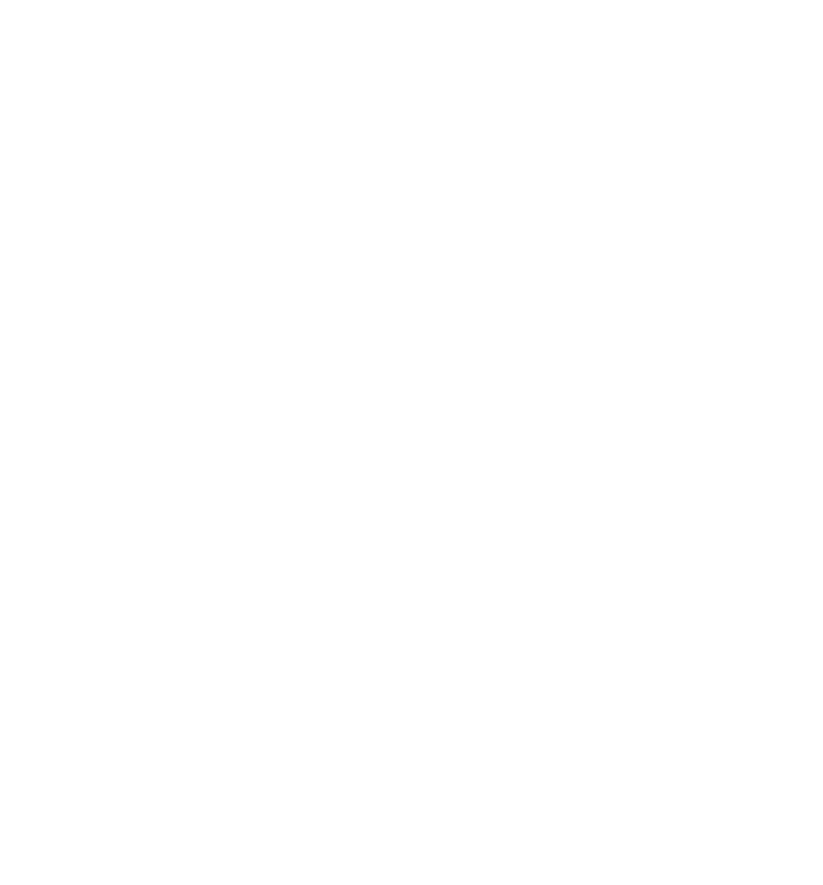
\includegraphics[height=0.3\textheight]{./Img/Experiment11_scheme_oneReceiver.pdf}
	}}
	\caption[Scheme of basic scenario]{Scheme of basic scenario with one noise source and one point of measure}
	\label{oneReceiverOneNSScheme}
\end{figure}

\begin{figure}
	\centering
	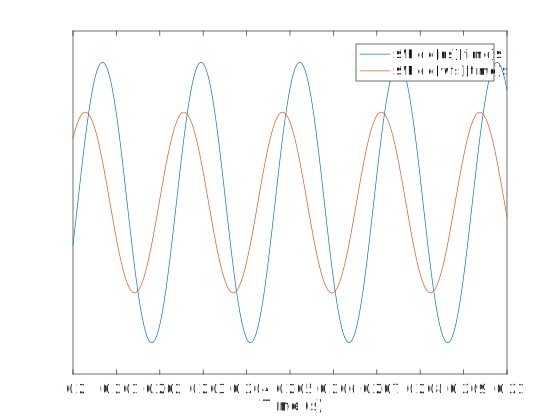
\includegraphics[width=0.4\columnwidth]{Img/Experiment11_exampleNoFreqCorr.eps}
	\caption{Signal measured}
	\label{oneReceiverPureDeltaReceived}
\end{figure}

In order to quantify the performance, we will use the concept of cancellation. It is a frequency dependent parameter, defined as the power of the signal received from the noise source divided by the power of the total signal ($\Field[total][frequency] = \Field[ns][frequency] + \Field[wfs][frequency]$). We will express it usually in dB:
\begin{equation}
\cancellation(f) = 20\log{\left\lvert\frac{\Field[ns][frequency](f)}{\Field[wfs][frequency](f) + \Field[ns][frequency](f)}\right\rvert}
\end{equation}
The maximum cancellation will happen when $\Field[ns][frequency] = -\Field[wfs][frequency]$.

Another useful parameter is what I call correction factor $\correctionFactor(f)$. It is conceived as the complex number by which loudspeakers signals $\signal[wfs][frequency]$ should be multiplied in order to achieve maximum cancellation:
\begin{equation}
\correctionFactor(f) = -\frac{\Field[ns][frequency](f)}{\Field[wfs][frequency](f)}
\end{equation}

In the previous case, the cancellation and corrections factors are $\cancellation = 3.6\si{dB}$ and $\correctionFactor = 1.1 e^{j40.3/360}$.

Since the aim of WFS is achieving cancellation over an wide area, it is reasonable to measure the field not in just one location, but in a grid of points, and the cancellation will vary from one to another. In that case, it is convenient come up with some way of describing the overall performance with just one value that takes in account the field at every point of measure. The concept of global cancellation can be used, defined as the overall measured power with the loudspeakers turned off divided by the overall total power:
\begin{equation}
\globalCancellation(f) = \frac{\sum_m \Field[ns][frequency][scalar][m](f)}{\sum_m \Field[total][frequency][scalar][m](f)}
\end{equation}

In the same way, the correction factor has a global equivalent, the global correction factor $\globalCorrectionFactor$, defined as the number that must be multiplied by the loudspeaker signals $\signal[wfs][frequency]$ in order to minimize the overall measured power.
\begin{equation}
\globalCorrectionFactor(f) = \argmin_{\psi} \norm{\psi \Field[wfs][frequency][vector] + \Field[ns][frequency][vector]}^2 = -\frac{\scalarProd{\Field[wfs][frequency][vector]}{\Field[ns][frequency][vector]}}{\norm{\Field[wfs][frequency][vector]}^2}
\end{equation}
where $\Field[wfs][frequency][vector] = [\Field[wfs][frequency][scalar][1],...,\Field[wfs][frequency][scalar][\numMeasPoints]]^T$ and $\Field[ns][frequency][vector] = [\Field[ns][frequency][scalar][1],...,\Field[ns][frequency][scalar][\numMeasPoints]]^T$.

So, instead of one point, now let's see what happens at a grid of points (\autoref{MultipleReceiverOneNSCanc}). It seems cancellation is bad at all of them. The global cancellation value is $\globalCancellation = 4.76 dB$. 

\begin{figure}
	\centering			\includegraphics[height=0.3\textheight]{./Img/Experiment11_multipleReceiverCancel2Dmap.eps}
	\caption[Cancellation 2D map]{Cancellation 2D map in dB}
	\label{MultipleReceiverOneNSCanc}
\end{figure}

It might be that the bad results have to do with the location of the noise source. Let's then see what happens for different positions as shown in \autoref{MultRecMultNSscheme}. Instead of just showing the 2D map of cancellations for each noise source positions, it will be more convenient for farther analysis to visualize it as a histogram of global cancellation values
\autoref{}.

\begin{figure}
	\centering
	\reflectbox{\rotatebox[origin=c]{180}{
			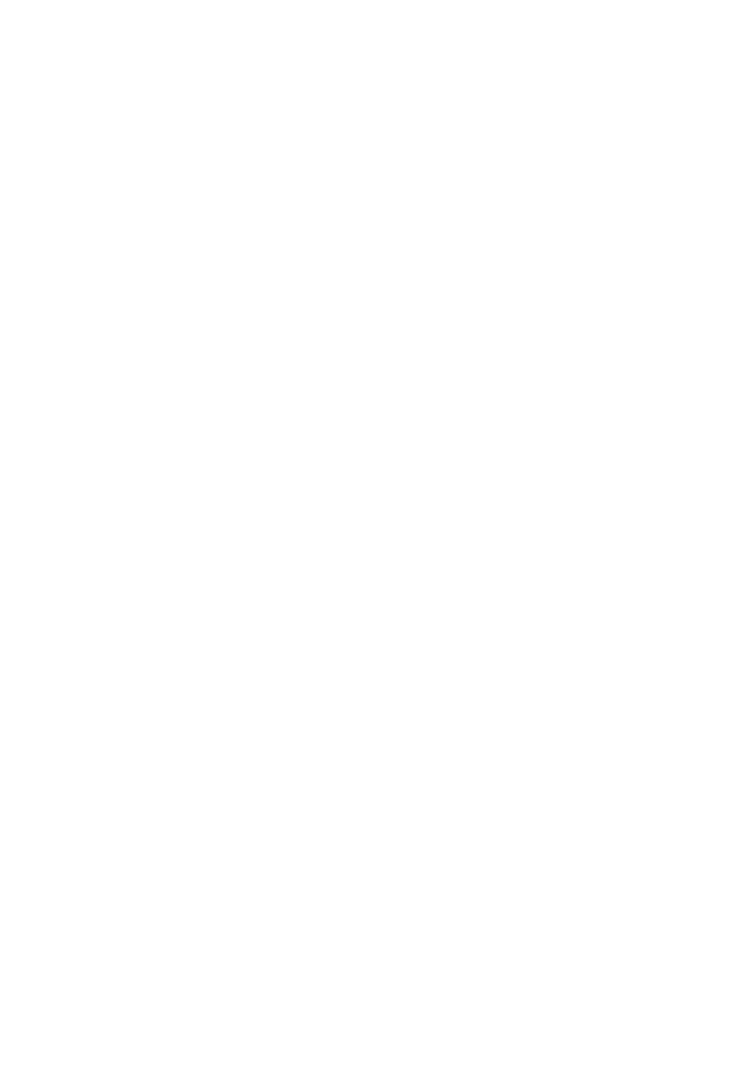
\includegraphics[height=0.3\textheight]{./Img/Experiment11_scheme_multipleReceiverMultipleNS.pdf}
	}}
	\caption[Scheme of multiple points of measure and multiple noise source positions]{Scheme of multiple points of measure and multiple noise source positions}
	\label{MultRecMultNSscheme}
\end{figure}

However, all this has been tested just at one frequency. Maybe, the behaviour for the rest of frequencies is different. To check it out, we will make the noise source transmit a chirp signal from $20 \si{Hz}$ to $940 \si{Hz}$ (close to the aliasing spatial frequency) and then calculate the FFT (for more information on how the simulations are carried out, consult appendix \autoref{appendixSimulation}). The global cancellation for the original noise source position is shown in \autoref{}. It is obvious that the values are bad over the whole bandwidth.

In order to understand what is happening for the whole bandwidth and multiple source position in just one snapshot, consider \autoref{}. It is the same histogram as in \autoref{}, but seen in 3D, and each bar has been coloured according to the height. If we look at it from above (\autoref{}), we won't appreciate the heigh, but the colour will be enough. That histogram is particularized for just one frequency ($440\si{Hz}$). If, for each frequency, we generate a similar coloured histogram and stack them next to each other, we can form an image as \autoref{} where the x axis is the frequency, the y axis is the cancellation value, and the colour is the ratio of occurrences in that interval; in other words, each column is a histogram of values.

\autoref{} tells us that the cancellation is bad at all frequencies, for every position of the noise source.

What is happening? The answer can be found if we represent the global correction factor $\globalCorrectionFactor$ (\autoref{}). We can see that, even when there is some variance between the values for different noise source positions, the overall tendency follows the theoretical expression $\sqrt{\frac{jk}{2\pi}}$ that was omitted for being considered unnecessary. This result suggests that it is indeed necessary.

The reason for this is that, even though that term is not necessary when generating wave fields that are going to be heard by humans, it is required when the aim is to interference destructively with another existing wave field. For example, for a noise field $\Field[ns][frequency] = 1$, the secondary source field should be $\Field[wfs][frequency] = -1$. But if the phase is shifted $-\pi/4$ ($1/\sqrt{j} = e^{-j\pi/4}$), the amplitude of the field is $|\Field[ns][frequency] + \Field[wfs][frequency]| = |1 - e^{-j\pi/4}| = 0.77$, which corresponds to a cancellation of $\cancellation = 2.32\si{dB}$. Amplitude variations of course also worsen the cancellation levels. So, the term $\sqrt{jk/2\pi}$ might irrelevant when for the human ear when listening to a signal, but are of vital importance if we are going to make a cancelling wave physically interfere with another. We can't get away with just ignoring it.

In conclusion, a $\sqrt{\frac{jk}{2\pi}}$ filter must be implemented in WFS when the intention is to perform active cancellation of noise. Theoretically the filter has an anticausal response, but it must be implemented as a FIR digital filter, so inevitably it will introduce some amount of delay that must be compensated \cite{Lapini2018}. That sets a constraint on how close the noise source can be to the loudspeaker array.